\chapter{Evaluierung der erstellten Modelle} % (fold)
\label{cha:eval_modell}

Im zweiten Teil der Evaluierung wird nicht der Umgang mit dem Werkzeug betrachtet (siehe dazu Kapitel \ref{cha:eval_werkzeug}), sondern auf das unmittelbare Resultat der Werkzeugverwendung, also das erstellte Modell eingegangen. Ebenfalls nicht Gegenstand der Untersuchung ist in diesem Abschnitt die Wirkung der Modellbildung auf die operative Arbeit („Production Work“), die in Kapitel \ref{cha:eval_aw} betrachtet wird.

Ausgehend von den erstellten Modellen und deren Entstehungsprozess wird also in diesem Kapitel untersucht, wie das Werkzeug auf die in dieser Arbeit gewählte Form der Unterstützung expliziter „Articulation Work“, nämliche der kooperativen Externalisierung und Abstimmung mentaler Modelle, wirkt. Dementsprechend sind die im folgenden Abschnitt beschrieben Hypothesen aus den Ausführungen der Kapitel über mentale Modelle (Kapitel \ref{cha:mentale_modelle}) und der Methodik zur Externalisierung derselben (Kapitel \ref{cha:methodik}) abgeleitet. 

Zusätzlich wird eine explorativ gebildete Hypothese untersucht, die sich auf inhaltlicher Ebene mit dem Phänomen der Abbildung von Zusammenhängen durch räumliche Konfiguration der Konzepte in einem Modell beschäftigt, das in der Untersuchung der Hypothese \ref{hyp:diagmodelle} bereits hinsichtlich der Werkzeugverwendung beschrieben wurde.

\section{Hypothesen} % (fold)
\label{sec:m_hypothesen}

In diesem Abschnitt werden die Hypothesen abgeleitet, die in diesem Kapitel geprüft werden. Wie in Kapitel \ref{cha:eval_werkzeug} ist zwischen konzeptuell aus der Aufgabenstellung bzw. der entwickelten Methodik abgeleiteten Hypothesen über die Wirkung des Werkzeugs und explorativ während der Evaluierung selbst gebildeten Hypothesen über Eigenschaften des Werkzeugs bzw. dessen Verwendung im Kontext der Modellbildung zu unterscheiden.

\subsection{Konzeptuell begründete Hypothesen} % (fold)
\label{sub:m_konzeptionell_begründete_hypothesen}

Die folgenden Hypothesen sind aus der Aufgabenstellung bzw. den Ausführungen zur Modellierungs-Methodik abgeleitet. Auf die entsprechenden Ausführungen in den Kapiteln \ref{cha:mentale_modelle} bzw. \ref{cha:methodik} wird jeweils bei der Begründung der Hypothesen verwiesen.

Ein wesentlicher Aspekt bei der Externalisierung mentaler Modelle ist die Offenheit der Repräsentationssprache. Diese ist aus Abschnitt \ref{sub:concept_mapping} begründbar und in Anforderung \ref{anf:nicht_vorgegebene_semantik_der_modellierungselemente} abgebildet. Unter „Offenheit“ ist in diesem Zusammenhang die Eigenschaft der Repräsentationssprache gemeint, keine vordefinierte Semantik der Modellelemente vorzugeben sondern diese von den Modellierenden festlegen zu lassen. Dies umfasst im vorliegenden Fall sowohl die Bedeutung der unterschiedlichen Konzepttypen als auch die Bedeutung der Verbindungen zwischen Konzepten. Das Werkzeug darf also in diesem Zusammenhang die Benutzer nicht bei der Wahl der Repräsentationskonzepte und damit bei der Externalisierung selbst einschränken.

\begin{hyp}
	\label{hyp:keine_einschränkung}
	Das Werkzeug schränkt Benutzer semantisch nicht bei der Externalisierung ihrer mentalen Modelle ein.
\end{hyp}

Das Argument der Nicht-Beschränkung der Benutzer bei der Externalisierung hat neben der eben beschriebenen Sprach-Dimension auch eine konkrete Modell-Dimension. Während sich obige Hypothese auf semantische Einschränkungen der Externalisieungsmöglichkeiten bezieht, ist sind auch konkrete, strukturelle Einschränkungen bei der Verwendung des Werkzeugs zur Externalisierung eines bestimmten mentalen Modells zu berücksichtigten. Die Externalisierung muss -- um nicht beschränkend zu wirken -- beliebig umfangreiche Modelle ermöglichen. „Umfangreich“ bedeutet hier, dass das Modell beliebig viele Elemente enthalten können muss und diese beliebig untereinander in Beziehung gesetzt werden können.
	
\begin{hyp}
	\label{hyp:beliebige_komplexität}
	Das Werkzeug ermöglicht die Repräsentation beliebig umfangreicher Modelle.
\end{hyp}

Die Externalisierung mentaler Modelle mit Hilfe von computer-gestützten Werkzeugen ist keine originäre Idee dieser Arbeit. Computerunterstützung existiert vor allem im Bereich des „Concept Mapping“ (siehe Abschnitt \ref{sub:concept_mapping}), das methodisch maßgeblich in das vorgeschlagene Vorgehen des hier vorgestellten Ansatzes einfließt (siehe Kapitel \ref{cha:methodik}). In den existierenden Werkzeugen werden jedoch die kooperative Erstellung und kommunikative Validierung der externalisierten Modelle nicht explizit berücksichtigt. Beide Aspekte sind jedoch -- wie bei der Beschreibung der Strukturlegetechniken REF ausgeführt -- wichtig für den Abgleich mentaler Modelle und damit für die erfolgreiche Durchführung von „Articulation Work“. Die Ermöglichung und Stärkung der Kooperation der Beteiligten untereinander ist also ein wesentlicher Teilaspekt der Anforderung \ref{anf:kollaborative_und_unmittelbare_manipulierbarkeit_des_modells} an das Werkzeug („Kooperative und unmittelbare Manipulierbarkeit des Modells“).

\begin{hyp}
	\label{hyp:stärkere_kooperation}
	Die Verwendung des Werkzeugs führt zu stärkerer Kooperation bei der Modellerstellung als die Verwendung von bildschirm-basierten Werkzeugen.
\end{hyp}

% subsection konzeptionell_begründete_hypothesen (end)

\subsection{Explorativ gebildete Hypothesen} % (fold)
\label{sub:m_explorativ_gebildete_hypothesen}

Im Verlauf der beiden Evaluationen war die Herstellung von Verbindungen zwischen Modellelementen aus technischen Gründen schwierig zu benutzen und sehr anfällig für Fehlfunktionen. Dies führte dazu, dass Verbinder nahezu nicht verwendet wurden (siehe dazu die Auswertungen zu Hypothese \ref{hyp:diagmodelle} in Abschnitt \ref{sub:repräsentation_diagrammatischer_modelle}). In dieser Situation wurden Beziehungen zwischen Modellelementen von den Benutzern durch die räumliche Anordnung der Elemente ausgedrückt. Diese implizite Darstellung von relationaler Information erfolgte in allen Fällen spontan und ohne Anleitung oder Instruktion. Dies führte zu der Vermutung, dass die Verwendung von Verbindern zur Abbildung von Beziehungen bzw. Zusammenhängen zwischen Elementen nicht notwendig ist. Um diese Vermutung zu prüfen, wurde sie formal als Hypothese \ref{hyp:keine_verbinder} in die Untersuchung aufgenommen.

\begin{hyp}
	\label{hyp:keine_verbinder}
	Zur Abbildung von Zusammenhängen ist die Verwendung von Verbindern nicht notwendig.
\end{hyp}

% subsection explorativ_gebildete_hypothesen (end)

% section hypothesen (end)

\section{Untersuchungsdesign und Durchführung} % (fold)
\label{sec:m_untersuchungsdesign}

In diesem Abschnitt wird auf Basis der oben formulierten Hypothesen das Untersuchungsdesign abgeleitet und die Durchführung der Untersuchung beschrieben. Der erste Teil des Abschnitts beschreibt die Operationalisierung der Hypothesen und damit die Festlegung wie diese konkret geprüft werden können. Im zweiten Teil des Abschnitts wird die Durchführung der Prüfung beschrieben. Hier erfolgt neben der Zuordnung der einzelnen Modellierungsblöcke (siehe Abschnitt \ref{sec:globales_untersuchungsdesign}) auch die Darstellung rein beschreibender Modell-Parameter, die nicht unmittelbar in die Prüfung der Hypothesen eingehen. 

\subsection{Operationalisierung} % (fold)
\label{sub:m_operationalisierung}

In diesem Abschnitt wird für jede Hypothese identifiziert, in welcher Form sie geprüft werden kann. Dies umfasst die Festlegung der Messpunkte sowie der jeweiligen Mess- und Auswertungsmethode (letzte bezugnehmend auf den in Abschnitt \ref{sec:eingesetzte_werkzeuge_und_verfahren} beschriebenen Verfahren). Zudem werden jene Evaluationsblöcke festgelegt, die für die jeweilige Untersuchung herangezogen wurden.

Für jede Hypothese wird also spezifiziert, anhand welcher Aspekte diese geprüft werden kann (= abhängige Variablen). Zudem wird festgelegt welche Ausgangssituation bei der Anwendung gewählt werden muss, um die Prüfung durchführen zu können (= unabhängige Variable) und welche Faktoren die Beurteilung ggf. ungewollt beeinflussen können (= Störvariablen).

\subsubsection{Keine semantische Einschränkung der Externalisierung} % (fold)
\label{ssub:keine_semantische_einschränkung_der_externalisierung}

Gegenstand dieses Abschnitts ist die Prüfung der Hypothese \ref{hyp:keine_einschränkung}. Diese bezieht sich auf die geforderte Eigenschaft des Werkzeugs, die Benutzer bei der Modellierung semantisch nicht einzuschränken.

Voraussetzung für die Prüfung dieser Hypothese ist die Verwendung des Werkzeugs zur Modellbildung bei einer Aufgabe, die die semantischen Kategorien der Strukturierung nicht vorgibt. In der eingesetzten Methodik wird die Festlegung von Elementtypen explizit gefordert (Vorgehen und Zeitpunkt dafür werden jedoch nicht vorgegeben). Etwaige Modellierungsvorkenntnisse können diese Festlegung insofern beeinflussen, als dass die Konzepte bekannter Sprachen bevorzugt eingesetzt werden könnten. Im Sinne der Hypothese ist dies jedoch keine Störvariable, da die Forderung nach nicht einschränkender Struktur auch die Verwendung existierender Modellierungssprachen umfassen muss.

Die nicht einschränkende Wirkung kann qualitativ anhand von Benutzeraussagen und dem Prozess und Ergebniss der Modellentstehung beurteilt werden. Im ersten Fall bieten sich neben der direkten Frage nach der Abbildbarkeit der gewünschten Information auch Teilaspekte des \gls{PMS}-Framework \citet{Sedera02} an, das unter anderem die subjektiv wahrgenommene Qualität des Modellierungsergebnisses und die Abbildbarkeit der subjektiv wichtigen Information im Modell in Fragebogen-Items codiert. Am Prozess- und Ergebniss der Modellentstehung selbst kann beurteilt werden, ob und inwieweit die zur Verfügung gestellten, semantisch nicht vorbelegten Modellierungselemente für die Abbildung der gewünschten Information ausreichend waren. Dazu kann betrachtet werden, ob die beschränkte Anzahl von Elementen im Verlauf der Modellierung zu verändertem Vorgehen in der Abbildung oder zur Nichtabbildung bestimmter Modellaspekte führte und ob durch semantische Mehrfachbelegung bzw. die Einführung von nicht als Modellierungselement vorgesehenen Bausteinen der Sprachumfang über das ursprünglich intendierte Maß hinaus erweitert wurde. 

Vergleichend können zusätzlich Modelle herangezogen werden, die aus identischen Fragestellungen wie jene mit dem Werkzeug erstellten resultieren, bei denen jedoch ein in der Anzahl und Semantik der Modellierungselemente frei erweiterbares Werkzeug zum Einsatz kommt. Hier ist von Interesse, ob die erstellten Modelle semantisch vielfältiger sind als jene, die mit dem hier vorgestellten Werkzeug erstellt wurden.

% subsubsection keine_semantische_einschränkung_der_externalisierung (end)

\subsubsection{Repräsentation beliebig umfangreicher Modelle} % (fold)
\label{ssub:repräsentation_beliebig_komplexer_modelle}

Gegenstand dieses Abschnitts ist die Operationalisierung der Hypothese \ref{hyp:beliebige_komplexität}. Dabei wird überprüft, ob das Werkzeug die Abbildung beliebig umfangreicher Modellierungsaufgaben ermöglicht.

Voraussetzung zur Prüfung dieser Hypothese ist die Verwendung von Modellierungsaufgaben, die zu Modellen unterschiedlichen Umfangs (d.h. mit unterschiedlich vielen Konzepten die unterschiedlich stark untereinander vernetzt sind) führen. Insbesondere die Abbildung von umfangreichen Modellierungsaufgaben (d.h. hier Aufgaben, die bei detaillierter Modellierung >15 Modellelemente benötigen\footnote{15 wurde als Grenze gewählt, weil diese Anzahl die Obergrenze an gleichzeitig am Werkzeug verwendbaren Elementen darstellt}) sind von Interesse. Etwaige Modellierungsvorkenntnisse der Benutzer sind bei der Prüfung dieser Hypothese nicht von Relevanz.

Die Repräsentation beliebig umfangreicher Modelle ist aufgrund der beschränkten Größe der Modellierungsoberfläche direkt an die Verwendung der Einbettungsfunktion des Werkzeugs gebunden. Mittels dieser können Teilmodelle in ein abstraktes Gesamtmodelle eingebunden werden, was eine beliebige Detaillierung der Modelle ermöglicht und damit die Abbildung umfangreicher Modelle erlaubt, deren Platzbedarf über die Größe der Modellierungsoberfläche hinaus geht. Das Ausmaß der Verwendung dieser Möglichkeit ist (bei geeignet umfangreichen Fragestellungen) also ein Maß für die  Eignung der Werkzeugs zur Abbildung umfangreicher Modelle. Daneben sind wiederum Aussagen der Benutzer über die Abbildbarkeit umfangreicher Modelle zur Prüfung der Hypothese heranzuziehen. Entsprechende Fragen wurden in den Modellierungsblöcken 2, 3, 4 und 5 gestellt, wobei die Fragestellungen in den Blöcken 2 und teilweise 4 eher zu einfachen Modellen, die auf der Oberfläche außreichend Platz fanden, führte und deshalb hier nicht berücksichtigt werden dürfen.

Vergleichend können wie bei der Prüfung der vorhergehenden Hypothese zusätzlich Modelle herangezogen werden, die aus identischen Fragestellungen wie jene mit dem Werkzeug erstellten resultieren, bei denen jedoch ein in der Anzahl und Semantik der Modellierungselemente frei erweiterbares Werkzeug zum Einsatz kommt. Hier ist im Gegensatz zu oben jedoch von Interesse, ob die erstellten Modelle umfangreicher sind als jene, die mit dem hier vorgestellten Werkzeug erstellt wurden.

% subsubsection repräsentation_beliebig_komplexer_modelle (end)

\subsubsection{Wirkung auf die Kooperation bei der Modellerstellung} % (fold)
\label{ssub:wirkung_auf_die_kooperation_bei_der_modellerstellung}

Gegenstand dieses Abschnitts ist die Operationalisierung der Hypothese \ref{hyp:stärkere_kooperation}. Gegenstand der Untersuchung ist hier, ob die Verwendung des Werkzeugs bei der Modellbildung zu stärkerer Kooperation zwischen den Beteiligten führt als der Einsatz von bildschirmbasierten Werkzeugen.

Die Prüfung der Wirkung des Werkzeugs auf die kooperative Abbildung von Modellen bedingt Fragestellungen, die Kooperation explizit einfordern. Etwaige Modellierungsvorkenntnisse beeinflussen die Prüfung der Hypothese nicht. Bei der Beurteilung zu berücksichtigen sind etwaige bestehende persönliche Bekanntschaften oder etablierte Gruppen, deren Zusammenarbeit bereits institutionalisiert ist. Um den Einfluss derartiger Faktoren möglichst auszuschließen, müssen die Gruppen bei der Modellbildung zufällig gebildet werden und etwaige Bekanntschaften innerhalb der gebildeten Gruppen explizit im Vorfeld der Untersuchung erhoben werden.

Die hier zu prüfende Hypothese baut auf Hypothese \ref{hyp:kollaborativ} auf. Dort war zu prüfen, ob das Werkzeug kooperatives Arbeiten grundsätzlich ermöglicht. In diesem Abschnitt wird geprüft, ob der Einsatz des Werkzeugs hinsichtlich der Kooperation der Beteiligten tatsächlich einen meßbaren Vorteil gegenüber einem traditionellen, bildschirmbasierten Werkzeug hat. Dazu ist es notwendig, eine vergleichende Untersuchung durchzuführen. Modellierungsblock 5 wurde dementspechend geplant und umfasste eine die kooperative Abbildung eines Modells sowohl am Modellierungstisch als auch mittels dem bildschirmbasierten Werkzeug CMapTools. Die Aufgabenstellung wurde so gewählt, dass das resultierende Modell grundsätzlich in beiden Werkzeugen abgebildet werden konnte. Untersucht wurde, in welchem Ausmaß Kooperation zwischen den beteiligten Personen auftrat. Als Metriken dienten dazu die Zeitverteilung der Beteiligung am Modellierungsvorgang, der Zeitanteil an Diskussion während der Modellbildung sowie die Anzahl der Initiativwechsel (Turn-taking) während eines Durchgangs.

% subsubsection wirkung_auf_die_kooperation_bei_der_modellerstellung (end)

\subsubsection{Abbildung von Zusammenhängen ohne Verbinder} % (fold)
\label{ssub:abbildung_von_zusammenhängen_ohne_verbinder}

Gegenstand dieses Abschnitts ist die Operationalisierung der Hypothese \ref{hyp:keine_verbinder}. Gegenstand der Untersuchung ist die Beobachtung, dass zur Abbildung von Zusammenhängen die Verwendung von explizit dargestellten Verbindern nicht notwendig ist.

Die Prüfung dieser Hypothese stellt keine Vorbedingungen an die Modellierungsaufgabe oder die Modellierungsvorkenntnisse der Benutzer. Auch können individuelle Anwendungen der Werkzeugs (d.h. nicht nur in kooperativen Szenarien) zur Untersuchung verwendet werden. 

Bei der Prüfung der Hypothese sind zwei Formen der Notwendigkeit von explizit dargestellten Verbindern zu unterscheiden. Zum Einen ist die Notwendigkeit bei der kooperativen Erstellung eines Modells zu untersuchen, bei der sämtliche Beteiligte zu einer einheitlichen Interpretation des dargestellten Modells kommen sollen. Zum Anderen muss auch der Fall einer zeitlich nachgelagerten Interpretation durch Dritte untersucht werden. Hier ist zu erheben, ob die Interpretation der Modellinhalts dem ursprünglichen Verständnis des bzw. der Modellierenden entspricht.

Zur Untersuchung muss dem ursprünglichen Modellierer jeweils eine inhaltliche Interpretation des Modellierungsergebnisses rückgespiegelt werden. Diese Form der kommunikativen Validierung kommt methodisch im Rahmen der Anwendung von Strukturlegetechniken (siehe Abschnitt \ref{sub:strukturlegetechniken}) zum Einsatz und ist deshalb ohnehin Teil der in dieser Arbeit vorgeschlagenen Methodik bei der kooperativen Anwendung des Werkzeugs. Zur zeitlich nachgelagerten Interpretation bedarf es einem separaten Schritt, in dem das Modellierungsergebnis von einer dritten, den der Modellierung nicht beteiligten Person interpretiert und rückgespiegelt wird. 

% subsubsection abbildung_von_zusammenhängen_ohne_verbinder (end)
% subsection m_operationalisierung (end)

\subsection{Durchführung} % (fold)
\label{sub:m_durchführung}

In diesem Abschnitt werden die für diesen Evaluierungs-Teil relevanten deskriptiven Parameter der berücksichtigten Anwendungs-Blöcke angeführt.
Als Grundlage der Überprüfung der Hypothesen werden hier die Evaluierungs-Blöcke 1 bis 5 verwendet. Dabei wurden für die quantitativ zu prüfenden Variablen die Blöcke 2 und 3 herangezogen, da in diesen die größten Stichproben zur Verfügung standen. In die qualitative Auswertung der Ergebnisse wurden hingegen alle Blöcke (1-5) mit einbezogen.

\subsubsection{Stichprobe} % (fold)
\label{ssub:stichprobe}

\begin{tabular}{| p{2cm} || p{2,5cm} | p{2,5cm} | p{2,5cm} || p{2cm} |}
  \hline
   & Aushandlung (1. Durchgang) & Aushandlung (2. Durchgang) & Concept Mapping & Gesamt \\ \hline
   $n_{Anwendungen}$ & 9 & 9 & 17 & 35 \\ 
   $n_{Teilnehmer}$ & 19 & 18 & 47 & 84 \\ \hline
\end{tabular} 

% subsubsection stichprobe (end)

\subsubsection{Modellgröße} % (fold)
\label{ssub:modellgröße}

Die Verteilung der Modellgröße wurde hier anhand der Anzahl der verwendeten Elemente (siehe Abbildung \ref{fig:img_Evaluierung_elementUsageBlocksOverview}) und der Anzahl der verwendeten Verbindungen (siehe Abbildung \ref{fig:img_Evaluierung_elementUsageConnectorsOverview}) dargestellt. Berücksichtigt wurden dabei die Ergebnisse der Modellierungsblöcke 2 („Aushandlung“) und 3 („Concept Mapping“). Die Modelle der Modellierungsblöcke 1 und 4 sind aufgrund der uneinheitlichen Aufgabenstellungen nicht vergleichbar, jener Teil des Modellierungsblocks 5, der mit dem hier vorgestellten Werkzeug durchgeführt wurden, weißt ob der identischen Aufgabenstellung hohe Ähnlichkeit mit den Ergebnissen von Block 3 auf.

\begin{figure}[htbp]
	\centering
		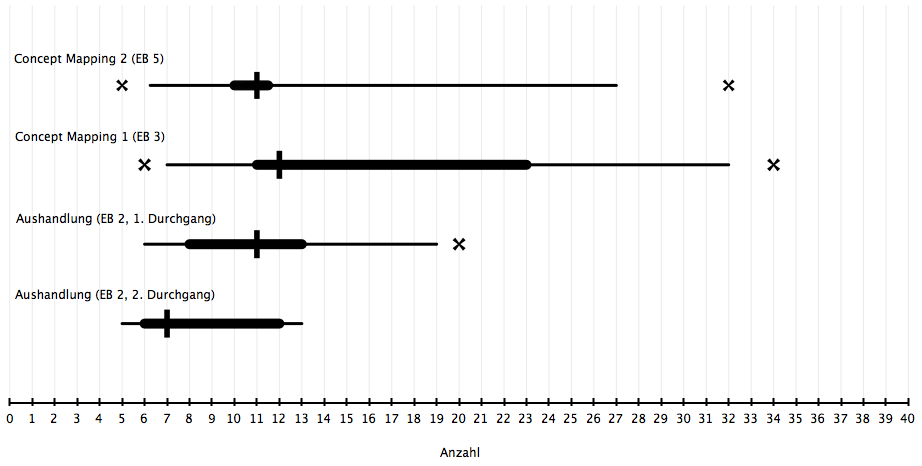
\includegraphics[width=15cm]{img/Evaluierung/elementUsageBlocksOverview.png}
	\caption{Anzahl der verwendeten Elemente -- Übersicht}
	\label{fig:img_Evaluierung_elementUsageBlocksOverview}
\end{figure}

In Abbildung \ref{fig:img_Evaluierung_elementUsageBlocksOverview} ist zu erkennen, dass der Median der Anzahl der verwendeten Elemente zwischen 7 und 12 liegt, wobei die Concept Mapping Aufgabe wegen des nicht explizit vorgegebenen Detaillierungsgrad der Modellierung eine höhere Schwankungsbreite (mit starker Tendenz zu größeren Modellen) aufweist. Zwar war der Detaillierungsgrad der Aushandlungsaufgaben ebenfalls nicht explizit vorgegeben, hier scheint jedoch eine höhere Überstimmung hinsichlich des angemessenen Detaillierungsgrades gegeben gewesen zu sein. 

Auffällig ist außerdem, dass zwischen den beiden Durchgängen des Aushandlungs-Blocks ein (statistisch allerdings wegen der geringen Stichprobengröße nicht signifikanter ($t=0.16 < t(0.95,8)=2.306$)) Unterschied in der Größe der Modelle (gemessen an der Anzahl der Elemente) gegeben ist. Dies scheint nach Betrachtung der qualitativ erhobenen Daten aus den entsprechenden Videoaufzeichnungen einerseits darauf zurückzuführen zu sein, dass der zweite Durchgang in einer späteren Phase des produktiven Arbeitsprozesses durchgeführt wurde, in dem weniger offene Schritte zu behandeln waren, andererseits scheint durch die bereits etablierte Zusammenarbeitsprozesse generell weniger Abstimmungsbedarf gegeben gewesen zu sein. Dieser Eindruck wird auch durch die generell geringere Modellierungdauer in Durchgang 2 (siehe Abbildung \ref{fig:img_Evaluierung_usageTimeNegotiation}) bestärkt.

\begin{figure}[htbp]
	\centering
		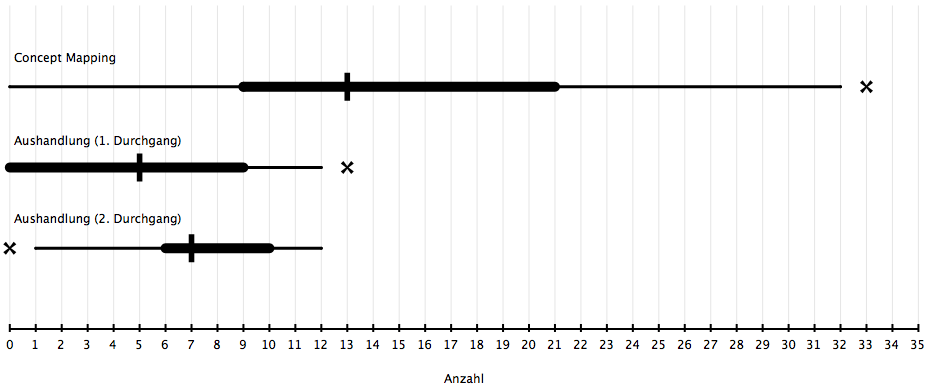
\includegraphics[width=15cm]{img/Evaluierung/elementUsageConnectorsOverview.png}
	\caption{Anzahl der verwendeten Verbindungen -- Übersicht}
	\label{fig:img_Evaluierung_elementUsageConnectorsOverview}
\end{figure}

Eine ähnliche Verteilung wie im Falle der Elemente ergibt sich bei Betrachtung der Anzahl der Verbindungen (siehe Abbildung \ref{fig:img_Evaluierung_elementUsageConnectorsOverview}). Auffällig ist jedoch die gegenüber Durchgang 2 des Aushandlungsblocks geringere Anzahl von Verbindungen in Durchgang 1 während sich die Anzahl der Blöcke zwischen den beiden Modellierungsdurchgängen umgekehrt verhält. Wie in der Überprüfung der Hypothese \ref{hyp:verbinder} in Abschnitt \ref{sub:herstellung_von_verbindern} bestätigt, ist dieses Phänomen auf die Fehlfunktionen und Instabilität der ursprünglichen Funktion zur Herstellung von Verbindungen zurückzuführen, die in Durchgang 1 ausschließlich zur Verfügung stand, während in Durchgang 2 (und auch im Block „Concept Mapping“) bereits die zusätzliche Funktion zur Verbindungsherstellung verfügbar war.

% subsubsection modellgröße (end)

\subsubsection{Vernetzungsgrad} % (fold)
\label{ssub:}

Der Vernetzungsgrad der Modelle („Connectedness“) wurde bereits zur Überprüfung der Hypothese \ref{hyp:verbinder} in Abschnitt \ref{sub:herstellung_von_verbindern} betrachtet, ist jedoch eine Eigenschaft der erstellten Modelle an sich und wird hier deshalb nochmals als deskriptiver Parameter beschrieben.

\begin{figure}[htbp]
	\centering
		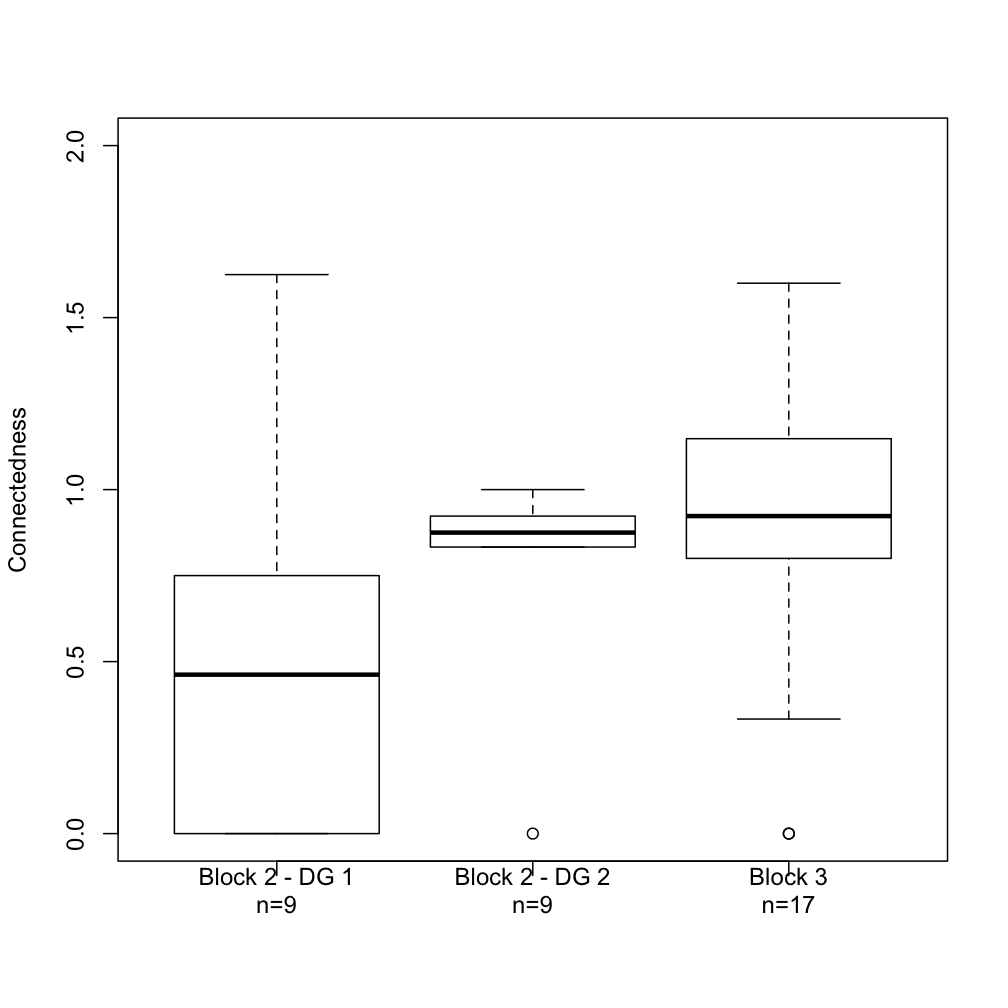
\includegraphics[width=10cm]{img/Evaluierung/connectednessOverview.png}
	\caption{Vernetzungsgrad (Verbindungen / Blöcke) -- Übersicht}
	\label{fig:img_Evaluierung_connectednessOverview}
\end{figure}

Abbildung \ref{fig:img_Evaluierung_connectednessOverview} zeigt die Verteilung des Verhältnisses der Anzahl von Verbindungen und Blöcken in den Modellierungsblöcken 2 und 3. Zu erkennen ist der oben und in Abschnitt \ref{sub:herstellung_von_verbindern} bereits beschriebene geringere Vernetzungsgrad im ersten Durchgang von Modellierungsblock 2 der auf die Instabilität und schwierige Verwendbarkeit der ursprünglichen Funktion zur Herstellung von Verbindungen zurückzuführen ist.

Seit der Verfügbarkeit der neuen Funktion zur Herstellung von Verbindungen (also im zweiten Teil von Block 2 sowie in den Blöcken 3, 4 und 5) liegt der Vernetzungsgrad im Mittel immer um 1, wobei in den letzten Blöcken (4 und 5) tendenziell noch höhere Vernetzungsgrade auftreten (Bock 4 im Mittel $1,32$, Block 5 im Mittel XY). Im Falle von Block 4 kann dies teilweise auf die Aufgabenstellungen zurückgeführt werden, die zum Teil starken Fokus auf die Repräsentation von Beziehungen legte (maximaler Vernetzungsgrad in einem Durchgang: $24/8=3$). Bei beiden Blöcken wurden außerdem weitere Stabilisrierungsmaßnahmen in der Interaktions-Erkennungsleistung des Systems vorgenommen, weshalb der gestiegene Vernetzungsgrad zum Teil auch auf die einfachere Herstellbarkeit von Verbindungen zurückgeführt werden kann (siehe wiederum \ref{sub:herstellung_von_verbindern}).

% subsubsection  (end)
% subsection m_durchführung (end)
% section untersuchungsdesign (end)

\section{Ergebnisse} % (fold)
\label{sec:m_ergebnisse}

\subsection{Keine semantische Einschränkung der Externalisierung} % (fold)
\label{sub:keine_semantische_einschränkung_der_externalisierung}

\subsubsection{Auswertung} % (fold)

\subsubsection{Diskussion} % (fold)

\subsubsection{Ergebnis} % (fold)

% subsection keine_semantische_einschränkung_der_externalisierung (end)

\subsection{Repräsentation beliebig komplexer Modelle} % (fold)
\label{sub:repräsentation_beliebig_komplexer_modelle}

\subsubsection{Auswertung} % (fold)

\subsubsection{Diskussion} % (fold)

\subsubsection{Ergebnis} % (fold)

% subsection repräsentation_beliebig_komplexer_modelle (end)

% subsection abstimmung_individueller_modelle (end)

\subsection{Wirkung auf die Kooperation bei der Modellerstellung} % (fold)
\label{sub:wirkung_auf_die_kooperation_bei_der_modellerstellung}

\subsubsection{Auswertung} % (fold)

\subsubsection{Diskussion} % (fold)

\subsubsection{Ergebnis} % (fold)

% subsection wirkung_auf_die_kooperation_bei_der_modellerstellung (end)

\subsection{Abbildung von Zusammenhängen ohne Verbinder} % (fold)
\label{sub:abbildung_von_zusammenhängen_ohne_verbinder}

\subsubsection{Auswertung} % (fold)

\subsubsection{Diskussion} % (fold)

\subsubsection{Ergebnis} % (fold)

% subsection abbildung_von_zusammenhängen_ohne_verbinder (end)
% section m_ergebnisse (end)

% chapter eval_modell (end)